\subsection{Развивающийся рынок (Китай)}
Теперь рассматриваем особенности развивающихся рынков, которые достаточно сильно отличаются от только что рассмотренных развитых.

Небезосновательно принято считать, что уровень риска на развивающихся рынках выше. Рассуждая глобально, замечаем, что утверждение логично, ведь для таких рынков не характерна стабильность, поскольку функционирование еще не отлажено рыночным механизмом и государственным содействием, а, следовательно, и уровень неопределенности существенно выше, чем на развитых рынках. Ещё в ключевой работе <<Риски, неопределенность, прибыль>> \cite{knight2003risk}  американский экономист Фрэнк Найт утверждал, что одним из основных источников неопределенности является изменение как таковое. Замечаем, что развивающиеся рынки как раз и синонимичны изменяющимся: появление новых игроков, меняющееся законодательство и в целом новизна явления для экономики страны. 

Сочетание нескольких факторов делает рынки более рискованными: низкий уровень развития биржевой инфраструктуры, несовершенная законодательная система, отсутствие прозрачности информации, а также превалирование государства в отдельных областях экономики. Эти факторы характерны для фондового рынка Китая, который к тому же начинал свою деятельность обособленно от мирового рынка, что в целом является характерной чертой для экономик Востока.

Азиатские рынки, тем более в настоящее время, представляют большой интерес для инвесторов по всему миру. Прежде всего интерес обусловлен наличием крупных экономик мира: помимо Китая, это Япония, Южная Корея, Индия. Развитие их финансовой системы хоть и началось существенно позже (приблизительно в середине XX века), однако продолжает совершенствоваться и производить привлекательный результат. Однако основной отличительной особенностью является вмешательство государства в регулирование системы. В том числе поэтому в некоторых странах замечена высокая концентрация активов в руках крупных компаний. Однако сложно говорить об оценке влияния государства, поскольку его деятельность необходима для обеспечения безопасности всех участников рынка, исполнения законодательства, реализации политики по стимулированию развития фондовых рынков. Именно государство вводит ограничения на финансовом рынке, которые помогают сохранить стабильность или предотвратить опасное падение. Несмотря на это развивающиеся рынки часто по-прежнему особенно неустойчивы.

Однако Китайский рынок ведет себя не совсем как типичный развивающийся рынок, хоть и имеет характерные черты. Пришло время рассмотреть его особенности. Отмечаем, что история создания и развития биржевой торговли в Китае началась еще в 1918 году, однако ввиду смены государственного строя и появлению национальной идеологии в 1949 биржи были закрыты. Возрождение фондового рынка \cite{berger2008fund} началось в 1990 --- 1991 гг. и требовалось не по естественным причинам перенаправления капитала в необходимые области, а скорее в рамках перехода страны к рыночной экономике. Законодательные изменения, внесенные в Конституцию в 2004 году, предоставили частной собственности главную позицию. И с этого момента начинается активное развитие реального сектора, и, как следствие, рынка ценных бумаг. Характерная для развивающихся рынков <<однобокость>>\footnote{Однобокость, в текущем случае, превалирование конкретной отрасли.} видна в первоначальном превалировании банков, однако она преодолевается грамотными рыночными реформами и политикой государства в отношении повышения активности на рынке акций и защите прав инвесторов. Выход ряда отечественных компаний на внутренние биржи повышает доверие населения и способствует дальнейшему развитию торговли ценными бумагами, а также некоторому перегреву, что сыграло важную роль в значительном падении индексов бирж в 2007 г. Отмечаем, что даже крупные компании не выдерживали, а просто потянули рынок за собой. Напоминаем, что б\'{о}льшая часть держателей акций --- частные инвесторы, причем не очень обеспеченные. Такое падение спровоцировало разорение большого количества участников рынков и способствовало снижению доверия. Волатильность рынка акций в первые годы работы бирж была зашкаливающей. В данном контексте можем рассмотреть текущую ситуацию с помощью ранее упомянутого China ETF Volatility \footnote{График построен на основе данных с сайта Investing.com URL: \url{https://goo.su/ZaOHV9}}, который отражает изменение цен на внутреннем рынке Китая. Его можно трактовать как оценку уровня риска при покупке отечественных Китайских акций.

\begin{figure}[H]
	\centering
	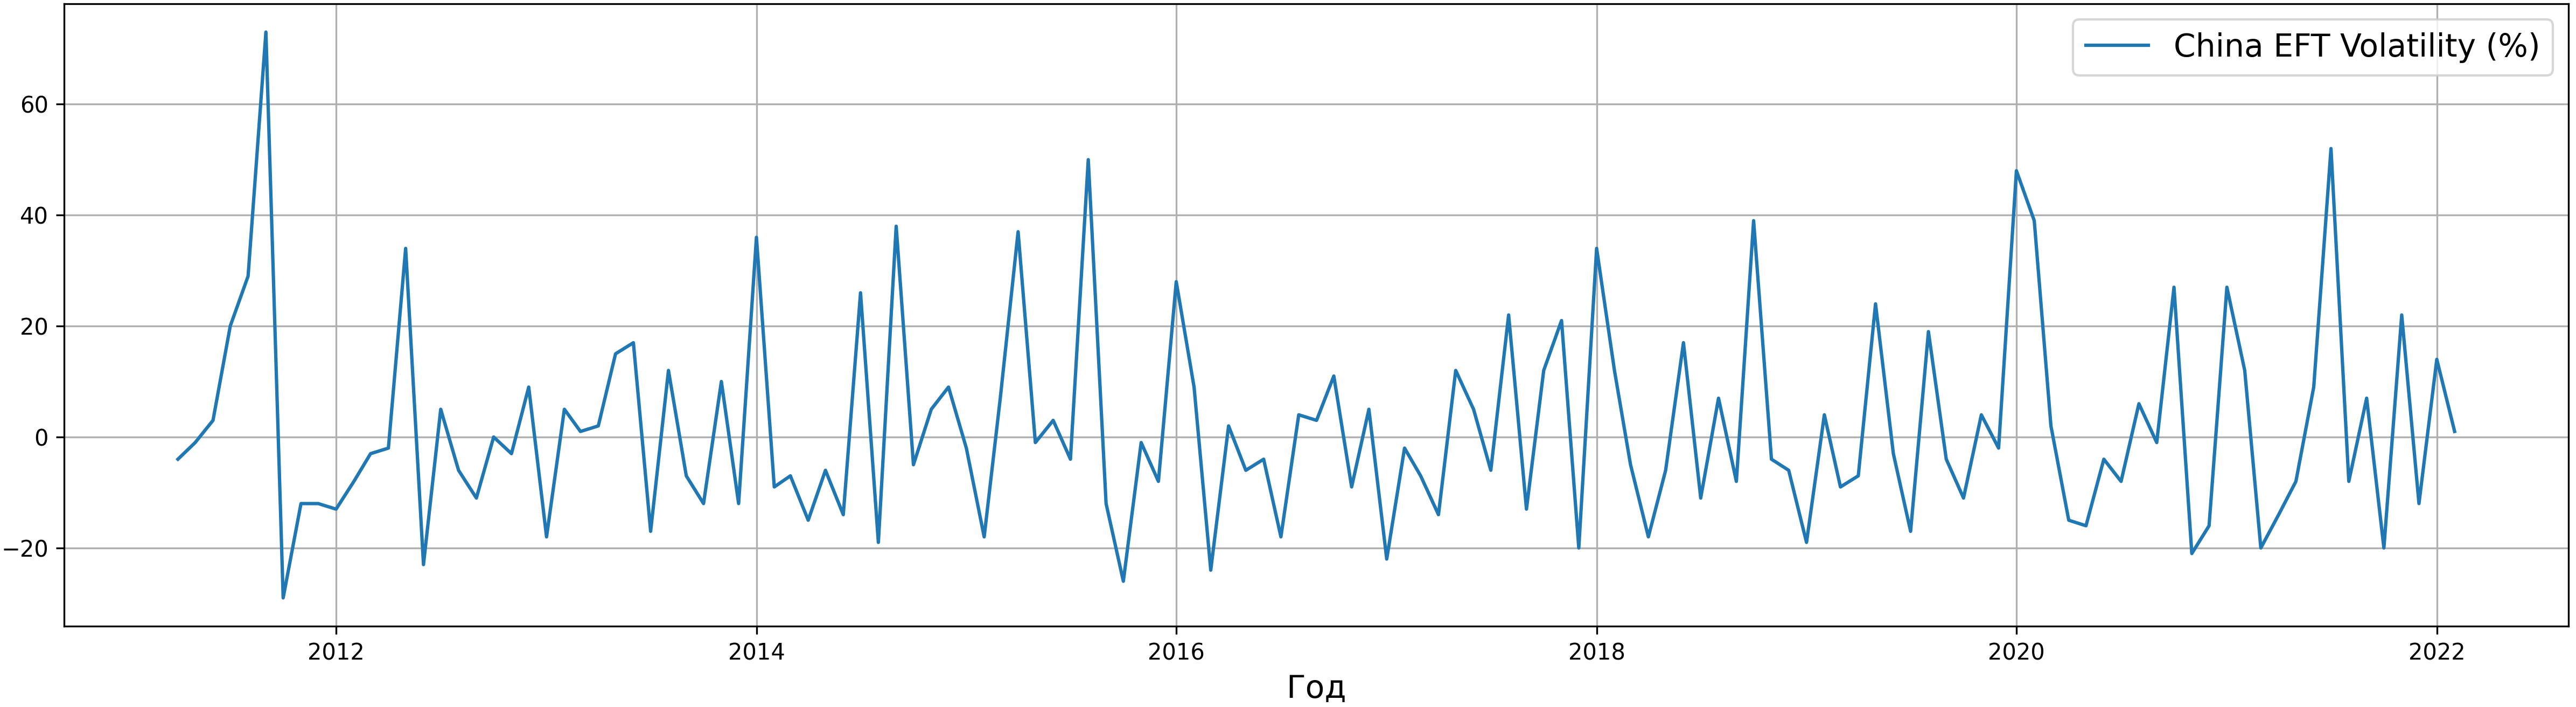
\includegraphics[width= 17cm]{market_data/developing_market/eft_china_volatility.png}
	\caption{Изменение China ETF Volatility}
\end{figure}

\noindent Как видно, что изменения цен достигают около 70\%, да и средний уровень достаточно высок. 

В связи с чем было введено немало регулирующих моментов \cite{hu2018chinese}. Для б\'{о}льшей стабильности было произведено разделение на отечественные (A-shares) и иностранные (B-shares) акции, а также прочие виды, которые упоминались ранее. Были введены несколько типов инвесторов, а также ограничение на приобретение акций отечественных компаний. Более того в Китае используются торговые ограничения, например, установление верхнего предела цены, по достижении которого торговля акциями возможна только на уровне цены, не превышающей предельный. Для предотвращения мошеннических операций, связанных с задержкой оплаты, также используется правило $T+1$, которое подразумевает зачисление средств и получение прав на акцию на начало следующего дня (рабочего, а не календарного) работы биржи. К компаниям, которые столкнулись с финансовыми трудностями или у которых наблюдается неконтролируемое поведение ценных бумаг, приписывается статус «Специального режима» и назначается вдвое меньший предел колебаний цен (5\%). Значимое ограничение касается иностранных инвесторов, желающих приобрести акции национальных китайских компаний. Помимо длительной процедуры регистрации и одобрения со стороны регулирующих органов, существуют ограничения в доле владения, ввиду которых иностранные инвесторы могут иметь небольшое количество акций, не позволяющее оказывать практически никакого влияния на управление. То есть фактически переводящее иностранных инвесторов в класс миноритарных, что может котироваться как все же дискриминация, недопустимая для развитых рынков.  Все это делает динамику цен акций не столь характерной для развивающихся рынков. 

Для б\'{о}льшей иллюстративности рассмотрим наглядные показатели, свидетельствующие о различиях в поведении рынков разных типов. Далее будут представлены данные о рыночной капитализации и среднегодовых доходностях.

Возможность оценки количественных характеристик предоставляет одно из крупнейших аналитических агентств в области международных инвестиций Morgan Stanley Capital International (далее MSCI) \cite{open2023family}, которые рассчитывают как различные индексы мирового масштаба, так и индексы странового уровня. Несмотря на то что данная работа проводится для распределения инвестиций фондов, данные могут быть использованы и для оценки экономического состояния среды.

Обращаем внимание на индекс MSCI Emerging Markets Index, который иллюстрирует индекс акций средних и крупных компаний развивающихся рынков для 25 стран \cite{investopedia2023emerging} с возможностью выбора конкретной страны. Отмечаем, что разделение стран на развитые и развивающиеся в практике MSCI не носит четких количественных рамок, а скорее основывается на экспертной оценке и сравнении \cite{investprovit2023developed}. Однако разделение публикуется каждый год в глобальном отчете. На 2022 год Китай, разделенный в классификации на China и China A, по-прежнему находится в списке развивающихся. При этом отмечается улучшение положения иностранных инвесторов на рынке акций типа A благодаря упрощению процесса подачи заявок и снижения требований к ним. Также повлияло и сравнительно недавнее создание опционов и фьючерсов, которое позволило использовать производные финансовые инструменты и на шаг приблизило внутренний рынок к пограничному (frontier) состоянию \cite{msci2022msci}. Однако короткие продажи не являются распространенной практикой и имеют существенные ограничения. Замечаем, что статус «развивающегося рынка» теперь утерян для России в силу событий февраля 2022 года, теперь мы причислены к категории «Остальные рынки», однако это произошло по б\'{о}льшей части в виду отсутствия доступа иностранных инвесторов к отечественным ценным бумагам.

\begin{figure}[H]
	\centering
	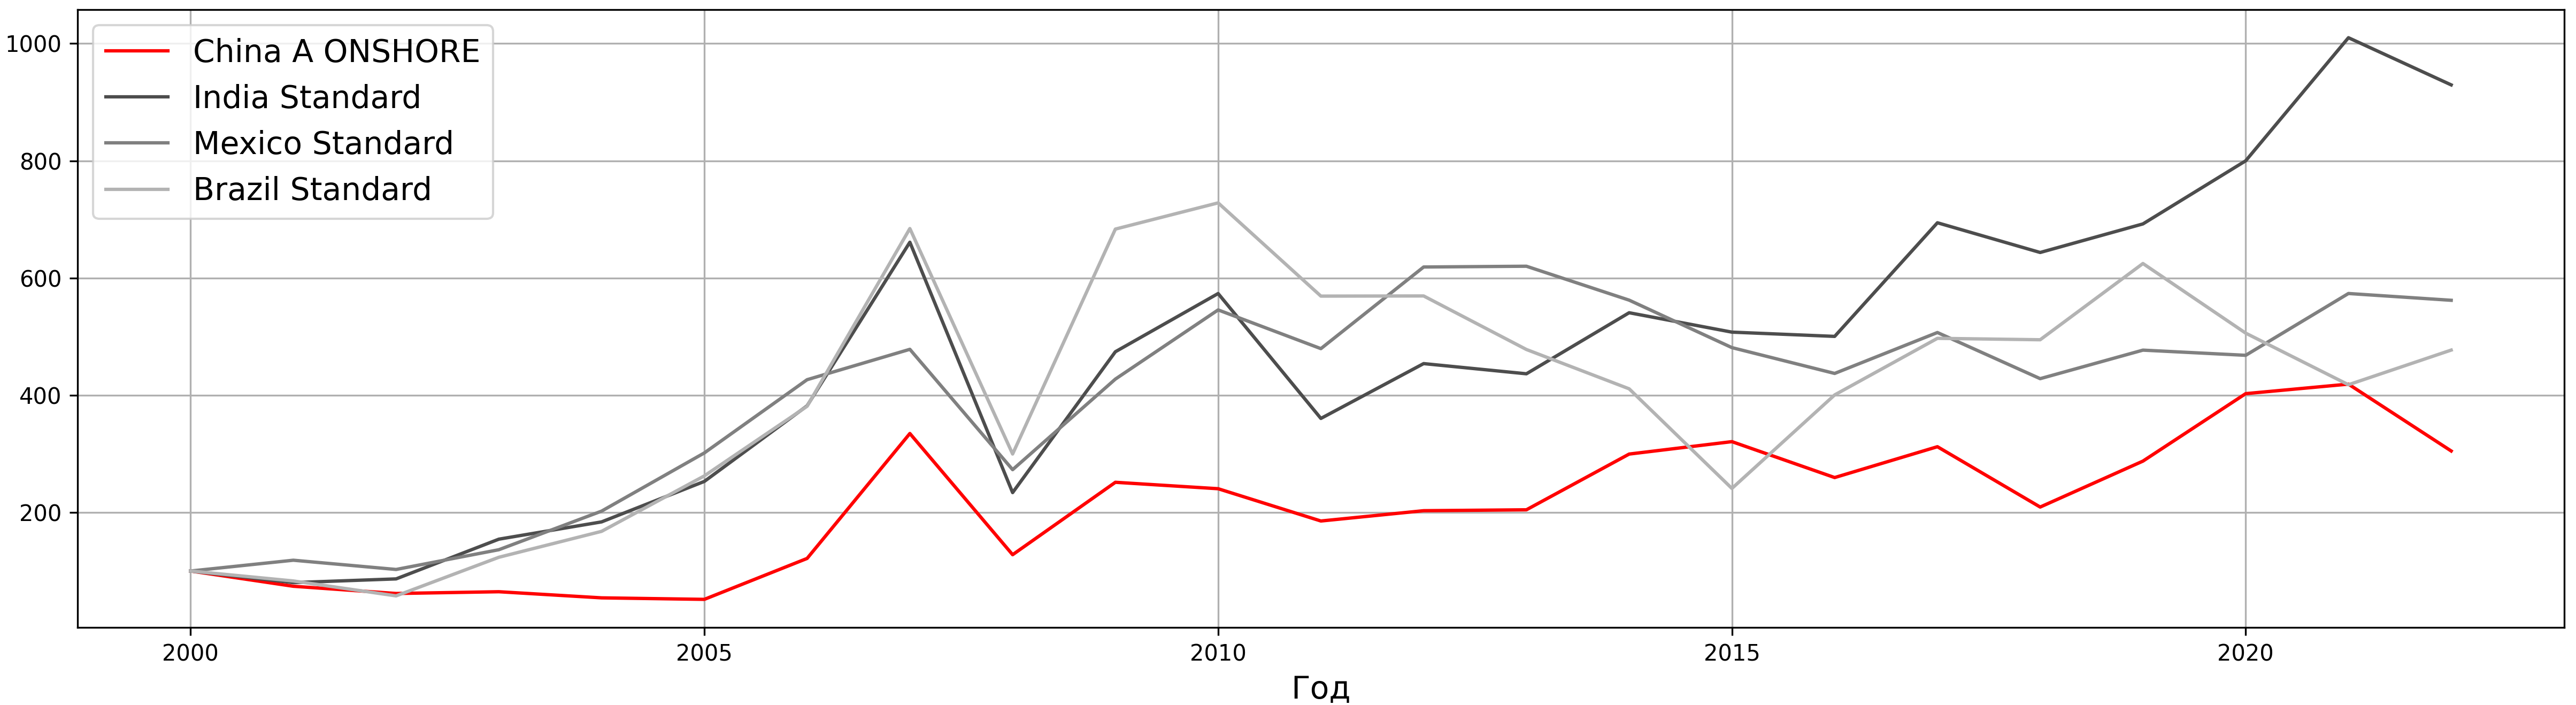
\includegraphics[width= 17cm]{market_data/developing_market/capitalization.png}
	\caption{Капитализация акций крупных и средних компаний нескольких развивающихся рынков, USD 2000 г. = 100\%}
\end{figure}

\noindent Итак, MSCI Emerging Markets Index показывает капитализацию по периодам (возможность выбрать: дни, месяцы, годы), фильтр позволяет выбрать конкретные регионы, а также посмотреть абсолютные значения и приросты (базис - первый год периода - принимается за 100) \footnote{График построен на основе данных агенства MSCI по капитализации развитых и развивающихся рынков. URL: \url{https://clck.ru/344z8Z}}. Что интересно, Китай, как уже говорилось ранее (даже с учетом только внутренних ценных бумаг) имеет самую высокую капитализацию среди развивающихся стран, однако, увеличивает ее сравнительно малыми темпами, что отражено на графике.

\begin{figure}[H]
	\centering
	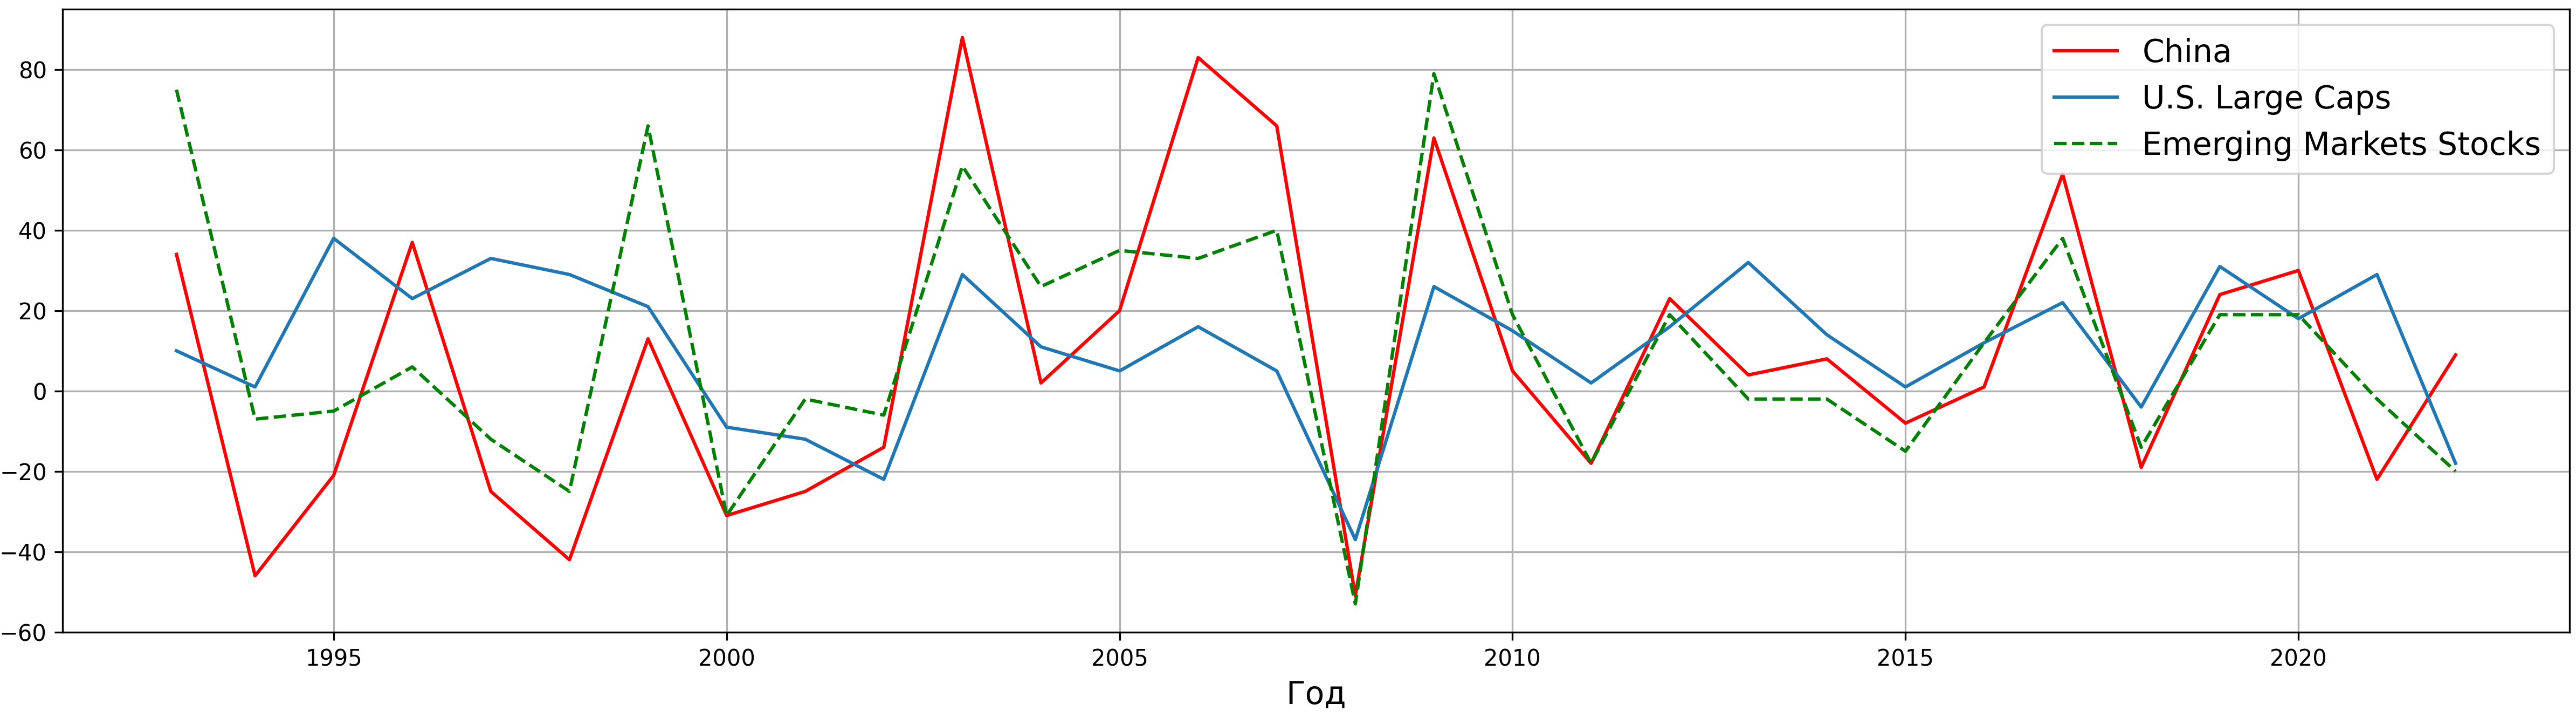
\includegraphics[width= 17cm]{market_data/developing_market/world_returns.png}
	\caption{Среднегодовая доходность фондового рынка США, Китая и развивающихся рынков (\%)}
	\label{pic::world_returns_last}
\end{figure}

\noindent Интересным представляется факт сравнения среднегодовых доходностей рынков. Обращаемся к графику (\ref{pic::world_returns_last}) \footnote{График построен на основе данных о MSCI Emerging Markets Indexes, 2023 URL: \url{https://goo.su/8fxzc}}, который отражает данную характеристику для Китая, США и в целом для развивающихся рынков. Хорошо видно, как активно увеличивалась среднегодовая доходность в период особой активности китайского рынка (2002 -- 2007), значительно превышая при этом доходность рынка США и среднюю доходность по развивающимся рынкам. Видим, что в целом амплитуда колебаний доходностей американских ценных бумаг существенно спокойнее фондового рынка Китай, значения доходностей на котором порою достигали 80\%, против 30\% в США.

